\documentclass[a4paper,10pt]{article}
\usepackage[paperwidth=210mm, paperheight=297mm, left=2.5cm, top=2.5cm, right=2.5cm, bottom=1.0cm, head=1.5cm, includefoot]{geometry}
%\usepackage[latin1]{inputenc}

\usepackage[english]{babel}
\usepackage[utf8x]{inputenc}
\usepackage{amsmath}

\usepackage{mathtools}
\DeclarePairedDelimiter\ceil{\lceil}{\rceil}
\DeclarePairedDelimiter\floor{\lfloor}{\rfloor}

\usepackage{bookman}
\usepackage{booktabs}
\usepackage[pdfborder={0 0 0}]{hyperref}
\usepackage{pdfpages}
\usepackage{fancyhdr}
\usepackage{lastpage}
\usepackage{verbatim}
\usepackage{graphicx}
\usepackage{fixltx2e}
\usepackage{listings}
\newsavebox{\codebox}% For saving code

%\usepackage[T1]{fontenc}
%\usepackage{comment}
%\usepackage{makeidx}
%\usepackage{float}
%\usepackage{slashbox}

\renewcommand{\headrulewidth}{1pt}
\renewcommand{\footrulewidth}{1pt}



%%%%%%%%%  Datos  %%%%%%%%%

\title{ \textbf{Trabajo práctico 2: Memorias caché} }

\author{Contini, Agustín - \textit{Padrón 89180}			\\
            \texttt{ agscontini@gmail.com }				\\
            Farina, Federico - \textit{Padrón 90177}			\\
            \texttt{ federicojosefarina@gmail.com }				\\
            Prystupiuk, Maximiliano  - \textit{Padrón 94853  }			\\
            \texttt{ mprystupiuk@gmail.com  }					\\[2.5ex]
            1er. Cuatrimestre de 2017					\\[1.0ex]
            \normalsize{66.20 Organización de Computadoras}		\\
            \normalsize{Facultad de Ingeniería, Universidad de Buenos Aires}	\\
	}
\date{\today}

%%%%%%%%%  Fin datos  %%%%%%%%%



\begin{document}



%%%%%%%%%  1era hoja: caratula y datos  %%%%%%%%%

\maketitle
\bigskip
\thispagestyle{empty}	% quita el numero en la primera pagina

\begin{abstract}
Familiarizarse con la medición de comportamiento utilizando herramientas
de profiling y con la estimación de parámetros de una memoria caché a partir de patrones de acceso y tasa de desaciertos al implementar una suite de
benchmarking de memorias caché.

\end{abstract}



%%%%%%%%%  Fin 1era hoja  %%%%%%%%%



%%%%%%%%%  Head y foot  %%%%%%%%%

\pagestyle{fancy}
\lhead{
\includegraphics[width=1.2cm]{./img/logo.png}}
\chead{Trabajo práctico 2: Memorias caché \\ \textit{Contini  -  Farina  -  Prystupiuk} }

\rfoot{$1^{er}$ Cuatrimestre 2017}
\lfoot{66.20 Organizaci\'on de Computadoras}
\cfoot{\hspace{2.4cm}   P\'agina \thepage \, de \pageref{LastPage} }

%%%%%%%%%  Fin head y foot  %%%%%%%%%



\normalsize

\newpage
\tableofcontents	% hoja de indices de titulos, subtitulos

\vspace{2.0cm}
%\listoffigures		% hoja de indices de figuras

\newpage
\section{Introducción}

\subsection{Herramienta utilizada}
Se utilizó Cachegrind, una herramienta del set de Valgrind que sirve para analizar la cache de una computadora simulando distinto tipos de cache y identificando la cantidad de referencias y cache misses sobre cada linea de codigo, función o sobre el programa entero.
\subsection{Desarrollo}
Se realizaron programas de benchmarking que reproducen el comportamiento del modelo de lazo simple.
Este modelo consiste en referenciar iterativamente una zona contigua de memoria. Cada bloque es referenciado en el mismo byte, siendo el salto entre las referencias de exactamente un bloque de caché.
\par
La cantidad de aciertos
y desaciertos en caché son conocidas en forma teórica. Para lazos más pequeños
que la caché que lo contiene, la tasa de desaciertos es cero, independientemente
de la configuración de esta. Cuando los lazos son más grandes, comienzan a
producirse desaciertos. Por ejemplo, para una caché de B bloques, si el lazo es
de un tamao entre B y 2B, las memorias caché asociativas por conjuntos con
LRU funcionan peor a medida que la asociatividad aumenta. Por lo tanto una
caché totalmente asociativa tiene la peor tasa de desaciertos y una asociativa
por conjuntos funciona mejor.
\par
Luego de utilizado este modelo de lazo se continuó con la medición de las distintas métricas ó en algunos casos solo fue utilizado como preparación inicial para una segunda prueba.

\newpage
\section{Parser}
\subsection{Descripción}
Parsea los datos del archivo de salida del modulo Cachegrind para que obtenga la tasa de miss de la memoria cache de datos y la guarda en un struct definido en el header \textbf{defines.h}. Este modulo permite el parseo de la ejecución de cada modulo de benchmarking a partir del nombre del módulo.



\section{Obtención del tamaño del bloque}
\subsection{Descripción}
Implementacion del modelo de lazo simple para obtener el tama~no del bloque de la memoria cache midiendo la tasa de miss que proporciona la herramienta parser desarrollada en el
módulo anterior. Se realizan los accesos más de una vez para poder despreciar el estado inicial de la cache.
\subsection{Desarrollo}
Se realiza un lazo escribiendo 1 MB, que por hipótesis se sabe es mucho mayor que el tamaño de la cache L1 de datos, de manera que todas las líneas de caché serán accedidas.
\par
Cómo todas las líneas fueron accedidas y sólo se produjo miss en el primer acceso a la línea, se puede calcular el tamaño de la misma:  
\[ \text{Tamaño de línea}
  = \dfrac{\text{Cantidad de veces que se accedió}}{\text{Cantidad de misses}}
\]

Para tener en cuenta el escenario en el que la cache sea WT realizamos lecturas para los accesos, lo que nos llevo a dividir numerador sobre 2 ya que es la cantidad de accesos realizadas para leer una posición del array en el módulo de benchmarking.
 
\section{Tamaño de la memoria caché}
\subsection{Descripción}
Módulo que ejecuta una implementacion del modelo de lazo
simple para obtenter el tamaño total de la memoria caché bajo estudio midiendo
la tasa de miss que proporciona la herramienta parser desarrollada
en un módulo anterior y usando el tamaño del bloque obtenido también en el anterior módulo de benchmarking.

Al igual que en el módulo anterior, se realizan los accesos más de una vez para poder despreciar el estado inicial de la cache.
\subsection{Desarrollo}
Se estima una cantidad inicial $N$ de bloques y se accede a dicha cantidad de bloques en la caché.
\par
Si para ese $N$ hay $N$ o menos misses quiere decir que quedaron bloques sin escribir.

Se aumenta en potencias de 2 dicho valor de $N$ hasta que sea mayor que la cantidad de misses, lo que significa que se están produciendo misses en las primeras posiciones de la caché nuevamente, con bloques ya escritos, por lo que se tendrá:
\[ \text{Tamaño de cache}
  = \dfrac{\text{N * Tamaño de Bloque}}{\text{2}}
\]


\section{Cantidad de conjuntos}

\subsection{Descripción}

Para esté módulo nos valdremos del cálculo anterior como estimación del tamaño de la cache y en base a eso se intentará estimar la cantidad de conjuntos en la que se divide la cache de datos.

Al igual que en los módulos anteriores, se realizan los accesos más de una vez para poder despreciar el estado inicial de la cache.

\subsection{Desarrollo}

Al igual que en el cálculo del tamaño de la cache se aumentara gradualmente el valor de $N$ iniciando con $N$=1, donde $N$ representará la cantidad de conjuntos.
Lo que se hará en este caso es realizar accesos a posiciones que tengan un offset del tamaño de la cache entre ellas y luego volver a leerlas a todas. Cuando se tenga, para un $N$, una cantidad de misses mayores a cero significará que el N ya supero en 2 veces la cantidad de conjuntos. Dicho esto el cálculo será:

\[ \text{Cantidad de conjuntos}
  = \dfrac{\text{N}}{\text{2}}
\]


\section{Executor}
\subsection{Descripción}

Este módulo será el encargado de correr los módulos de benchmarking presentes. Al igual que el parser, recibe como parámetro el nombre del módulo. Luego, desde el main del proyecto, cada uno de los módulos será ejecutado y su output será parseado lo que le dará al usuario un retorno por sálida standard.

\section{Corridas de prueba}

\begin{figure}[h!]
	\centering
	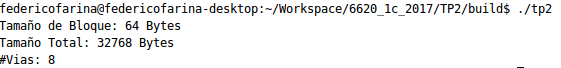
\includegraphics[width=1.0\textwidth]{./pruebas/default.png}
	\caption{Prueba usando cache sin simulación}
    \label{fig:default}
\end{figure}


\begin{figure}[h!]
	\centering
	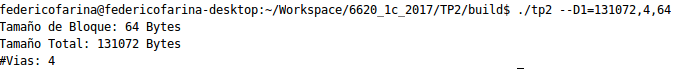
\includegraphics[width=1.0\textwidth]{./pruebas/D1_131072_4_64.png}
	\caption{Prueba simulando cache}
    \label{fig:default}
\end{figure}


\begin{figure}[h!]
	\centering
	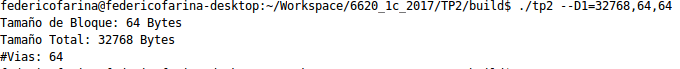
\includegraphics[width=1.0\textwidth]{./pruebas/--D1_32768_64_64.png}
	\caption{Prueba simulando cache}
    \label{fig:default}
\end{figure}


\section{Compilación y uso}
\subsection{Compilación}

El proyecto está basado en cMake. El build de todos los módulos se obtiene conjuntamente con los siguientes pasos:

\begin{enumerate}
\item  Copiar la carpeta TP2 y ejecutar:
	\begin{verbatim}
$ mkdir build && cd build
$ cmake .. && make && ./tp2
	\end{verbatim}
\end{enumerate}

\subsection{Opciones de uso}
\begin{enumerate}
\item  Parametros
	\par
    \text{-h, –help}
    \par
    \text{-v, –version}
    \par
    \text{-D1=Tamaño, vas, bytes x lnea}
\end{enumerate}

\section{Conclusión}

Si bien el TP estuvo orientado al conocimiento de la cache y a las maneras de estimar su composición con distintos módulos de benchmarking pudimos aprender e interactuar con herramientas de profiling muy poderosas que podríamos usar en otro contexto para optimizar o evaluar la performance de cualquier programa agnosticamente de lenguaje y la plataforma elegida.

\section{Código fuente}
\label{sec:code}

\subsection{Main}
\lstset{ language = C, numbers=left, tabsize=4, breaklines=true, frame=single }
\lstinputlisting{./source/main.cpp}

\subsection{Definiciones}
\lstset{ language = C, numbers=left, tabsize=4, breaklines=true, frame=single }
\lstinputlisting{./source/defines.h}

\subsection{Parser}

\lstset{ language = C, numbers=left, tabsize=4, breaklines=true, frame=single }
\lstinputlisting{./source/parser.cpp}

\lstset{ language = C, numbers=left, tabsize=4, breaklines=true, frame=single }
\lstinputlisting{./source/parser.h}

\subsection{Executor}

\lstset{ language = C, numbers=left, tabsize=4, breaklines=true, frame=single }
\lstinputlisting{./source/moduleExecutor.cpp}

\lstset{ language = C, numbers=left, tabsize=4, breaklines=true, frame=single }
\lstinputlisting{./source/moduleExecutor.h}

\subsection{Tamaño de bloque}

\lstset{ language = C, numbers=left, tabsize=4, breaklines=true, frame=single }
\lstinputlisting{./modules/blockSize.cpp}

\subsection{Tamaño de cache}

\lstset{ language = C, numbers=left, tabsize=4, breaklines=true, frame=single }
\lstinputlisting{./modules/cacheSize.cpp}

\subsection{Cantidad de conjuntos}

\lstset{ language = C, numbers=left, tabsize=4, breaklines=true, frame=single }
\lstinputlisting{./modules/cacheAssociativity.cpp}




\end{document}
